\section{Method and experimentation}
\label{sec:method}
In this section we detail our method for sensitive content detection in video. We split our approach into three parts: feature extraction, feature fusion and feature classification, as illustrated in Figure \ref{fig:model}.
\begin{figure*}[!ht]
    \centering
    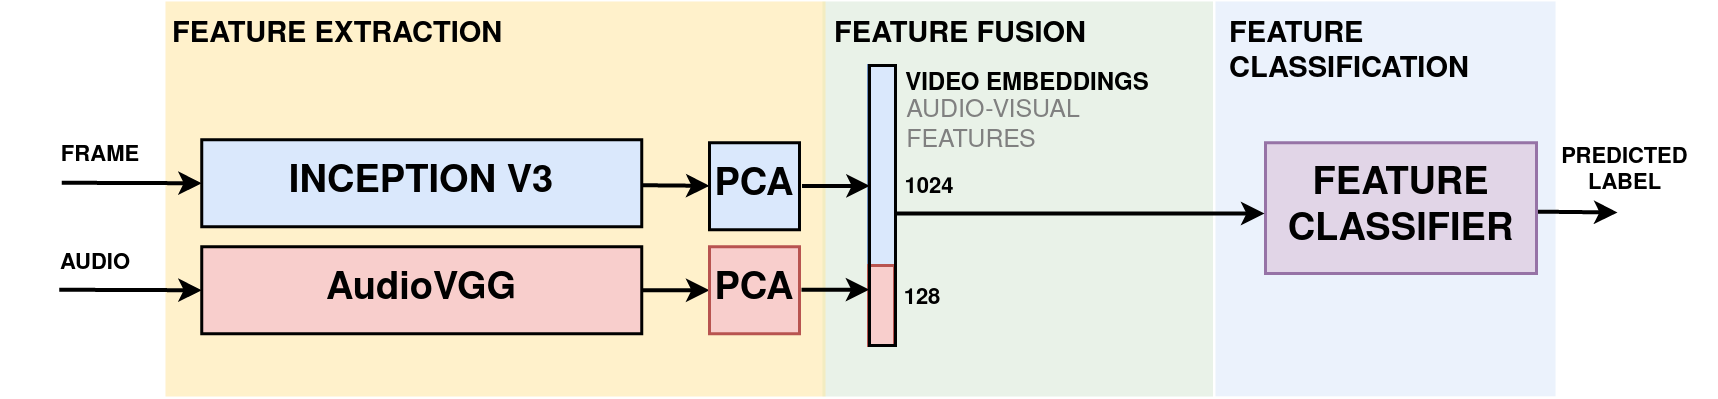
\includegraphics[width=0.9\textwidth]{img/model-2.png}
    \caption{Bimodal architecture for NSFW video classification.}
    \label{fig:model}
    \vspace{-1em}
\end{figure*}

In the feature extraction stage, firstly we split the frames and audio from the video; then, for each media, we use a CNN to extract the features (or embeddings) from each simultaneous video segment. In the second stage, Feature Fusion, we concatenate both audio and frame features. If the classification model is not sequential, we also aggregate the features in this stage. Finally, in the feature classification stage we feed one of the classification models to be experimented with.

\subsection{Video Embeddings Extraction}
\label{subsec:video_features}

CNNs tend to learn low-level features (\textit{e.g.}, in the visual domain: edges, corners, contours) at their first layers. At the intermediate and final layers, the combination of these features helps to extract more complex features, resulting in a vector of continuous values, referred to as \textit{embeddings}, that might be used for classification and other tasks. In this work, we use two benchmark CNNs to extract both image and audio \textit{embeddings} by using a transfer learning technique~\cite{tan2018survey}.



%Afterwards, we apply PCA (+ whitening) to reduce feature dimensions to 1024, followed by quantization (1 byte per coefficient).
%These two compression techniques reduce the size of the data by a factor of 8. The mean vector and covariance matrix for PCA was computed on all frames from the Train partition. We quantize each 32-bit float into 256 distinct values (8 bits) using optimally computed (non-uniform) quantization bin boundaries. We confirmed that the size reduction does not significantly hurt the evaluation metrics. In fact, training all baselines on the full-size data (8 times larger than what we publish), increases all evaluation metrics by less than 1%.

\todo{explicar pq escolheu as cnns (youtube) e qual foram os paramretros usados (pca e hiperparametros)}
By using the feature extraction method created for the Youtube-8m benchmark, we can test an feature extraction method that is powerful enough to represent features that can be in multiple tasks, such as multi-label video classification, video recommendation, and human activity recognition.

"Since the video-level representations are unsupervised (extracted independently of the labels), these representations are far less specialized to the labels associated with the current dataset, and can generalize better to new tasks or video domains."~\cite{abu2016youtube}

In order to validate our dataset, we used the same feature extraction method used in the Youtube-8m dataset challenges~\cite{abu2016youtube}, both networks were pre-trained and frozen and they were not retrained for application sensitive content classification. Which gives future works an opportunity to develop even more efficient and smaller feature extraction networks for this specific task.


To generate image frame features and audio features we decode each video at approximately 1 frame-per-second and feed an InceptionV3  network~\cite{szegedy2016rethinking} pre-trained on the ImageNet\footnote{\url{http://www.image-net.org/}} dataset.
 
We also make use of a AudioVGG~\cite{hershey2017cnn} network with pre-trained weights in the Audioset\footnote{\url{https://research.google.com/audioset/}} dataset to extract the audio embeddings. Each of these CNNs were used as published by their authors; the only modification was the removal of classification layers in both CNNs to obtain their respective embeddings.

Next, we apply Principal Component Analysis (PCA)~\cite{wold1987principal} to each of the outputs to reduce the dimensions of both embeddings and to generate feature vectors of size 1024 and 128 for frame and audio embeddings respectively.
%DETALHAR MAIS AQUI DE QTO PRA QTO O PCA REDUZ

\subsection{Feature Fusion}
\label{subsec:feature_fusion}

Once we have the features from both image and audio, we should make a decision about which method is best to fuse the information from these different domains. Snoek et al. \cite{snoek2005featurefusion} presents two main strategies for information fusion in semantic video analysis: \emph{Early fusion} methods, which works directly with the extracted features, and \emph{Late fusion} methods, which operates on classification outputs from specialized models.
%\todo{For a more recent survey about data fusion and multimedia retrieval, please refer to \cite{jiang2013features}.}
In this work, because we have high abstraction level features, we opted to investigate the most simple approach, which is to use a single model on the concatenated features from both media inputs.

Specifically, we concatenate both image and audio embeddings extracted in the current frame and audio window in order to compose the final embeddings as a sequence of the same size of the number of seconds of the video. After this concatenation, each time-step has 1,152 features: 128 audio features and 1024 frame features.

Notice that with this approach, the video is transformed into a time series, and to use it in non-sequential models (\textit{e.g.}~SVM, KNN, and MLP) we need to turn this sequence into a single feature vector that represents the whole video. In our setting, we did that by taking the average, median, standard deviation, min, and max values for each feature to represent the entire video. In summary, we turn the sequence of features with size $n$ and shape $n$ by 1,152 into a single feature with shape 1 by 5,760.

\subsection{Classifiers}
\label{subsec:classifiers}

% \todo[inline]{porque foi escolhidos esses modelos de classficação, qual a relação deles com o nosso tipo de dado de vídeo.}

For the feature classification task, we will investigate both sequential models (which use the extracted embeddings in a time series format), and non-sequential ones (which use a single aggregated embeddings vector).
We want to experiment with both approaches in order to investigate if a more compact format, such as the single embeddings vector, can yield results at least as good (or even better) than the full feature sequence data.
%Furthermore, we can test if a sequential model can outperform a non-sequential model in specific cases that demand long term memory, such as long videos with very small sensitive scenes.
As an example, one can think of a long video that has a pornographic scene in one second out of its entirety. 
In a non-sequential representation of the extracted features, this short pornographic fragment could be left ``hidden'' among the other non-pornographic frames of the video, as illustrated in Figure \ref{fig:model-non-sequence}.
\begin{figure*}[!ht]
    \centering
    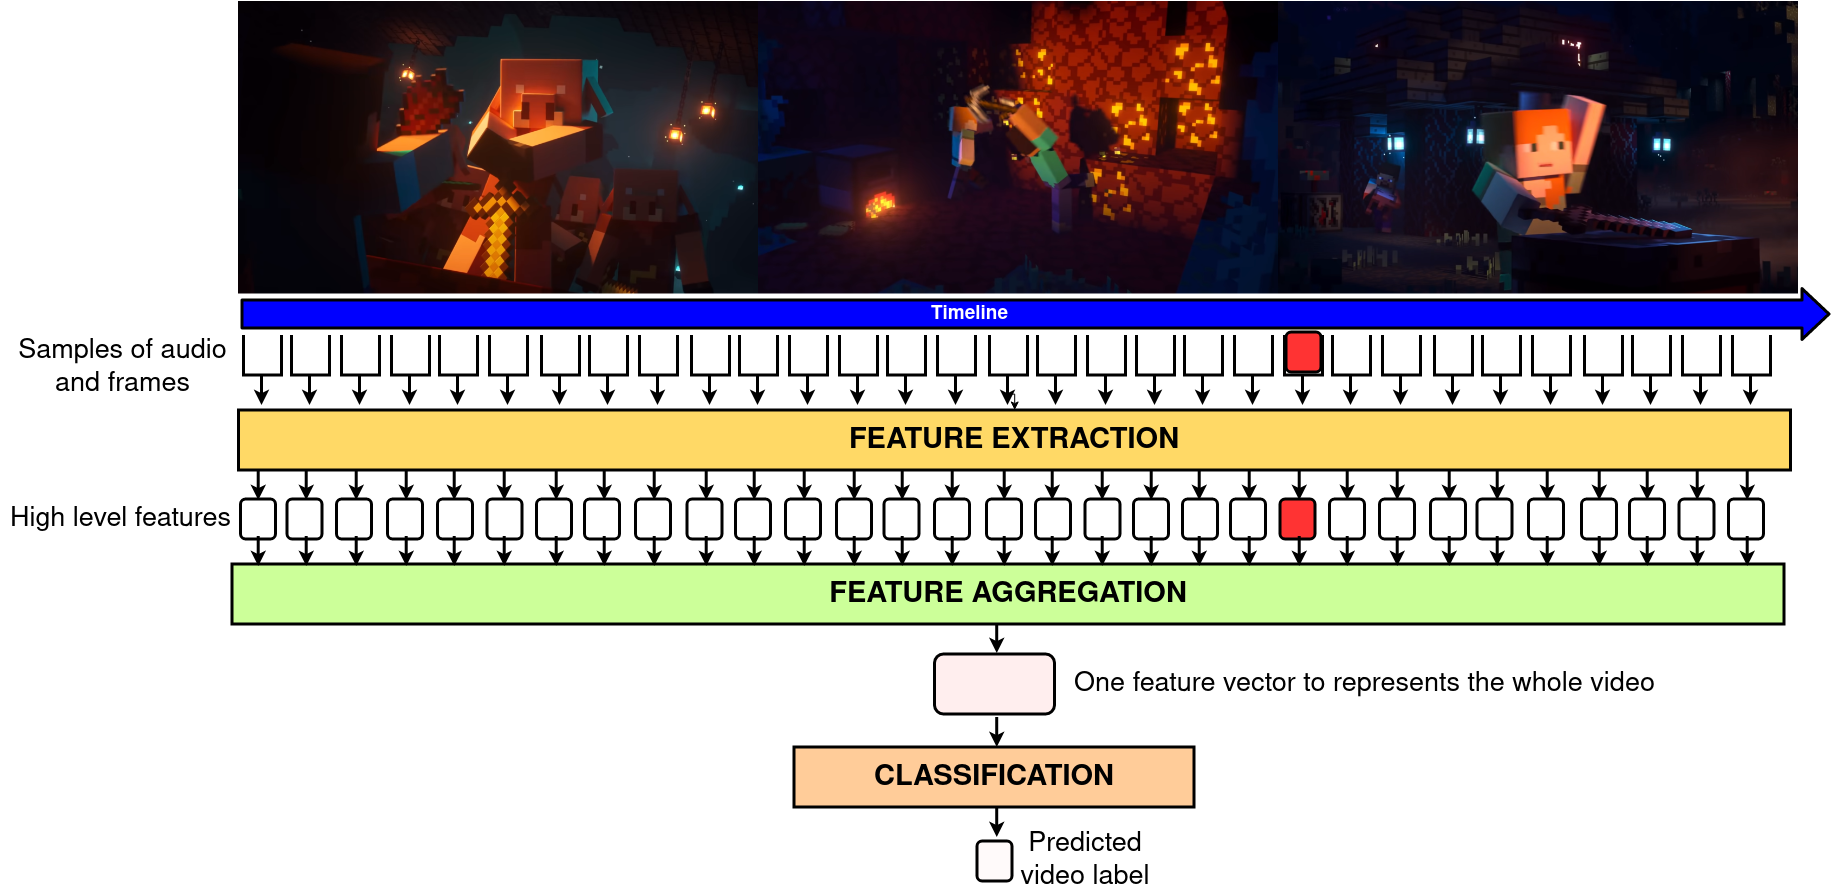
\includegraphics[width=0.9\textwidth]{img/model-non-sequence.png}
    \caption{Sequential features with aggregation, the sensitive scene (red) might vanish among the the other scenes during aggregation.}
    \label{fig:model-non-sequence}
    \vspace{-1em}
\end{figure*}
In a sequential representation, although time series classifiers usually output a prediction after reading the entire sequence, the embedding vectors of each second of the video would not be aggregated and thus could be analysed section by section, as illustrated in Figure \ref{fig:model-sequence}.

\begin{figure*}[!ht]
    \centering
    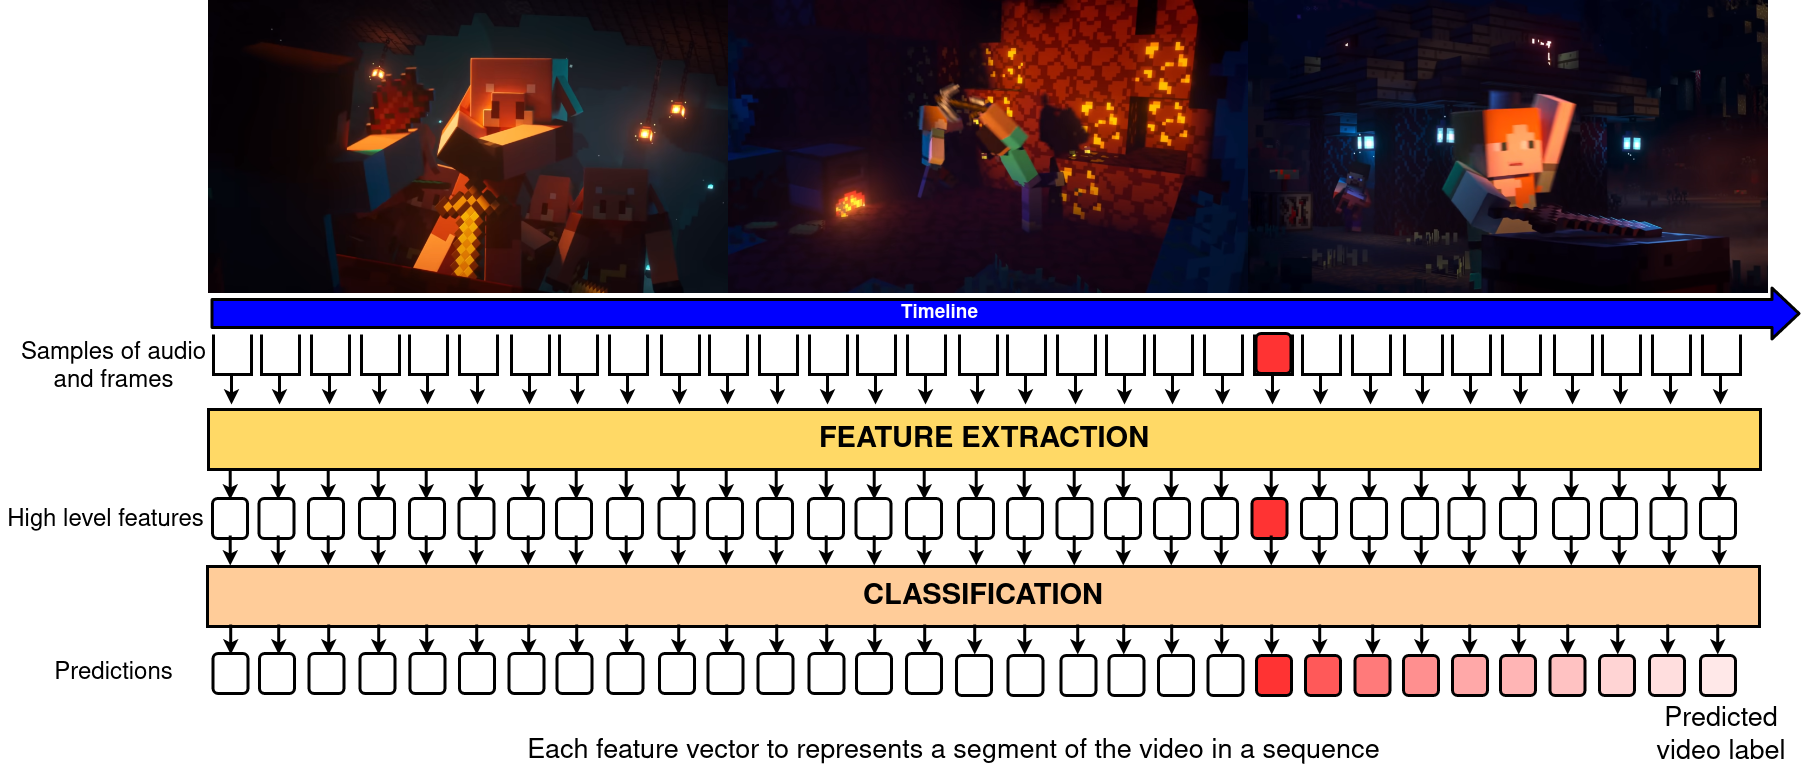
\includegraphics[width=0.9\textwidth]{img/model-sequence.png}
    \caption{Sequential features with no aggregation. In a output after reading the entire sequence, this can also be susceptible to information vanishing.}
    \label{fig:model-sequence}
    \vspace{-1em}
\end{figure*}
Although a sequential representation contains possibly much more redundant data than the non-sequential one, it could give the sequential classification model an important edge of detail over the less granular non-sequential ones.
% To do the feature classification task, we experimented four well known classification mohave dels, one using extracted video features in the time series format, and three that use a single aggregated feature vector.

For the sequential classification model, we chose the Long Short-Term Memory (LSTM)\cite{hochreiter1997long} networks.
It has been a commonly used time series classification baseline model. %\todo{mayber say we'll test GRUs?}

For the non-sequence models, we chose Support Vector Machines (SVM)~\cite{cortes1995support}, K-Nearest Neighbors (KNN)~\cite{peterson2009k}, and Multilayer Perceptron (MLP)~\cite{haykin2009neural}.
Among all of the experimented models, the \textit{Support Vector Machine (SVM)} is the most used in the literature.
% \begin{enumerate}[leftmargin=*]
% \item 
It is a classification model in which the data is mapped into a higher dimension input space, where an optimal separating hyper-plane is constructed.
% These decision surfaces are found by solving a linearly constrained quadratic programming problem.
% \item 
The second model, \textit{K-Nearest Neighbors (KNN)} uses distance measure between training samples so that the k-nearest neighbors always belong to the same class, while samples from different classes are separated by a large margin. 
It was chosen because it used also by related work, although it is a simple classification method.
% \item 
The third model is the \textit{Multilayer-perceptron (MLP)}, which contains layers of nodes: an input layer, an output layer and various hidden layers in between. 
This one was selected because it is also commonly used as a final classifier on deep neural networks.  
% The number of layers used is problem dependent, as is the number of nodes in each hidden layer.
% The weights are adjusted by local optimization using a set of feature vectors so that the network produces the optimal expected output.
% \item 
%Lastly, \textit{Long short-term memory (LSTM)}, different than the feed-forward neural networks, process the entire sequences of data using feedback connections.
% \end{enumerate}

In next the Section, we present the \textit{dataset} created to train and evaluate these classification models.

\section{Dataset}\label{sec:dataset}
% Falar do sampling inicial, da presentatividade dos sets
% falar do balanceamento e do sampling do conjunto de teste
% Falar das talbeas no texto
% colocar o resto das tabelas talvez no appendix
% estatisticas depois de dropar os maiores e os menores videos, sem balanceamento
% usamos o balanceamento dropando apesa porn videos pq os gore sao poucos
% iremos distribuir o dataset na versao balanceada e sem balanceamento
% Comparar nossas escolhas de corte de tempo com o do yt 
% Checked for duplicates by name and size and by fdupes, sem garantias de de não ter subvideos


% Before clipping video based on duration
% Mean:  0:06:18.929511  STD:  0:12:18.237458
% There are 1355 (1.05%) videos longer than 00:30:56
% There are 116 (0.09%) videos shorter than 00:00:05

% Videos:
% Total dataset: 127075
% Total size of videos (calculated individually): 3.5TiB
% Total duration of videos (calculated indiviadually): 11806:21:13
% Improper videos: 67424
% Total size of videos (calculated individually): 1.2TiB
% Total duration of videos (calculated indiviadually): 6953:27:41
% Proper videos: 59651
% Total size of videos (calculated individually): 2.2TiB
% Total duration of videos (calculated indiviadually): 4852:53:31
% Total size of features: '896.3GiB'

% Hot much detail do we go on about the dataset's subclasses? (subclasses por porn and yt, no subclasses on gore)

Our \textit{dataset} is structured into two main classes: videos containing ``safe'' content and videos containing sensitive content.
It is divided into 59,651 safe videos and 67,424 videos with sensitive content.

\begin{table}
\centering
\label{tab:general-stats}
\caption{General statistics of the two main classes of the dataset, tag coverage refers to main tag annotation existence (videos may also have sub tags but no main tag).}
\begin{tabular}{c|r|r} 
\multicolumn{1}{l|}{} & Sensitive  & Safe        \\ 
\hline
Video Count           & 67424      & 59651       \\ 
\hline
Total Duration        & 6953:27:41 & 4852:53:31  \\ 
\hline
Mean Duration         & 00:06:11   & 00:04:52    \\ 
\hline
STD Duration          & 00:04:12   & 00:03:26    \\ 
\hline
Max Duration          & 00:30:55   & 00:30:55    \\ 
\hline
Min Duration          & 00:00:05   & 00:00:05    \\ 
\hline
Total Size            & 1.2TiB     & 2.2TiB      \\ 
\hline
Mean Size             & 19.3MiB    & 39.0MiB     \\ 
\hline
STD Size              & 35.4MiB    & 42.3MiB     \\ 
\hline
Features Size         & 519.4GiB   & 376.8GiB    \\ 
\hline
Tag coverage          & 65392      & 51011       \\ 
\hline
Tag coverage (\%)     & 96,9862    & 85,5157     \\
\end{tabular}
\end{table}
% \subsection{SFW Videos}\label{sec:safe_videos}

For \textit{safe content}, we extracted 50,988 videos from Youtube8M\footnote{\url{https://research.google.com/youtube8m}}~\cite{abu2016youtube}. We chose this dataset because of the size of the dataset (8 million videos) and because of the wide variety of video classification challenges it supports.

We also included 8,663 videos collected from Youtube, hereby refered as cherry-picked, those videos were selected for the purpose of incremeting the amount of "hard" videos, which are videos that could possibly be misclassified as sensitive, such as MMA, breastfeeding, pool party, beach and other videos that have a higher amount of skin exposure. The amount of cherry-picked videos collected are listed by its query in Table \ref{tab:non-yt-count}. The collection was made by automated means, an script automatically searches and downloads all videos from the first 100 result pages.
% One of the objectives of the project is to evaluate the presence of inappropriate videos in educational video repositories. Therefore, in selecting your own videos within YouTube8M, we have chosen videos from \ "Jobs \& Education" and "News" top-categories.
% We made this choice because these videos generally have the "talking head" format. We believe that this format is common in an educational video repository such as video@RNP.
% \footnote{\url{https://video.rnp.br}}.

% We also included the Cholec80 \cite{twinanda2016endonet} dataset, it contains 80 videos of cholecystectomy surgeries performed by 13 surgeons. All videos from the Cholec80 dataset were labeled as safe, since videos of surgery are usual in an educational context.

% \subsection{NSFW Videos}\label{sec:nsfw_videos}

For \textit{sensitive content}, we collected pornography and violent videography (thereafter referred to as \textit{gore}) from websites. For the porn category, we collected 54,549 videos from XVideos\footnote{\url{https://info.xvideos.com/db}}. We chose this source because of the database size (7 million videos) and because of the amount and variety of annotations. In this database, each video has one main tag, totalling 70 main tags, and none or many subtags (user-created). To select the videos in this database, we distributed videos in these tags to maintain a proportion equal to the original XVideos database. In particular, to prevent lower-quantity tags from disappearing, we have defined a minimum of 10 pornographic videos for each tag. 

For the gore content, we used a web crawler to extract 2,356 gore videos from various websites dedicated to gore media, such as, BestGore\footnote{\url{https://www.bestgore.com/}} and GoreBrasil\footnote{\url{https://www.gorebrasil.com}}. 

%\todo{o set de teste de gore n tem gore de verdade, incluir?}
%For testing purposes we collected a separate group of 671 violent videos from youtube channel BustedLocals\footnote{\url{https://www.youtube.com/channel/UCpKimtjklYBgSKfSJrnXLRA}}
\begin{table}
\centering
\label{tab:granular-stats}
\caption{Granular statistics of the dataset: Videos collected from Youtube, pornographic videos, and gore videos.}
\begin{tabular}{c|r|r|r} 
\multicolumn{1}{l|}{} & \multicolumn{1}{c|}{Porn} & \multicolumn{1}{c|}{Gore} & \multicolumn{1}{c}{YouTube}  \\ 
\hline
Video Count           & 65068                     & 2356                      & 59651                         \\ 
\hline
Total Duration        & 6900:17:38                & 53:10:02                  & 4852:53:31                    \\ 
\hline
Mean Duration         & 00:06:21                  & 00:01:21                  & 00:04:52                      \\ 
\hline
STD Duration          & 00:04:10                  & 00:01:26                  & 00:03:26                      \\ 
\hline
Max Duration          & 00:30:55                  & 00:16:56                  & 00:30:55                      \\ 
\hline
Min Duration          & 00:00:05                  & 00:00:05                  & 00:00:05                      \\ 
\hline
Total Size            & 1.2TiB                    & 15.8GiB                   & 2.2TiB                        \\ 
\hline
Mean Size             & 19.8MiB                   & 6.9MiB                    & 39.0MiB                       \\ 
\hline
STD Size              & 35.9MiB                   & 13.9MiB                   & 42.3MiB                       \\ 
\hline
Features Size         & 515.3GiB                  & 4.1GiB                    & 376.8GiB                      \\ 
\hline
Tag coverage          & 63036                     & 2356                      & 51011                         \\ 
\hline
Tag coverage (\%)     & 96,8771                   & 100,0000                  & 85,5157                       \\
\end{tabular}
\end{table}

We hold out our dataset for testing and validating our approach: 10\% of the safe videos, then 10\% of gore videos, and sample a number of pornography to to match the amount of safe videos minus the amount of gore test samples, so that the test subset has a balanced amount of sensitive and safe videos, while keeping a valid amount of gore videos. 

\begin{table}
\centering
\label{tab:subset-stats}
\caption{Test subset statistics.}
\begin{tabular}{c|r|r|r} 
\multicolumn{1}{l|}{} & \multicolumn{1}{c|}{Safe} & \multicolumn{1}{c|}{Pornography} & \multicolumn{1}{c}{Gore}  \\ 
\hline
Video Count           & 5968                      & 5732                             & 236                        \\ 
\hline
Total Duration        & 443:35:36                 & 574:03:29                        & 05:22:20                   \\ 
\hline
Mean Duration         & 00:04:27                  & 00:06:00                         & 00:01:21                   \\ 
\hline
STD Duration          & 00:02:32                  & 00:03:44                         & 00:01:48                   \\ 
\hline
Max Duration          & 00:29:01                  & 00:30:29                         & 00:16:56                   \\ 
\hline
Min Duration          & 00:00:07                  & 00:00:05                         & 00:00:07                   \\ 
\hline
Total Size            & 204.8GiB                  & 80.2GiB                          & 1.5GiB                     \\ 
\hline
Mean Size             & 35.1MiB                   & 14.3MiB                          & 6.6MiB                     \\ 
\hline
STD Size              & 35.0MiB                   & 25.6MiB                          & 14.4MiB                    \\ 
\hline
Features Size         & 34.5GiB                   & 42.6GiB                          & 424.1MiB                   \\ 
\hline
Tag coverage          & 5679                      & 5695                             & 236                        \\ 
\hline
Tag coverage (\%)     & 951.575                   & 993.545                          & 100                        \\
\end{tabular}
\end{table}


As a complementary test dataset, we selected the NPDI 2k-pornography dataset~\cite{avila2013pooling}, it contains 1000 non-pornographic videos and 1000 pornographic videos. Those non-pornographic videos are comprised of ``hard'' and ``easy'' videos according to the likelihood of misclassification. Some examples of ``hard'' videos are those with high amounts of exposed skin, such as swimming and sumo fighting videos.

\begin{table}
\centering
\label{tab:2kdataset-stats}
\caption{NPDI 2k-pornography dataset statistics.}
\begin{tabular}{c|r|r} 
\multicolumn{1}{l|}{} & \multicolumn{1}{c|}{Porn} & \multicolumn{1}{c}{Non-Porn}  \\ 
\hline
Video Count           & 1000                      & 1000                           \\ 
\hline
Total Duration        & 100:30:32                 & 40:26:06                       \\ 
\hline
Mean Duration         & 00:06:01                  & 00:02:25                       \\ 
\hline
STD Duration          & 00:05:49                  & 00:02:17                       \\ 
\hline
Max Duration          & 00:33:40                  & 00:20:16                       \\ 
\hline
Min Duration          & 00:00:05                  & 00:00:02                       \\ 
\hline
Total Size            & 26.4GiB                   & 18.5GiB                        \\ 
\hline
Mean Size             & 27.0MiB                   & 18.9MiB                        \\ 
\hline
STD Size              & 31.1MiB                   & 21.9MiB                        \\ 
\hline
Features Size         & 7.6GiB                    & 3.1GiB                         \\ 
\hline
Tag coverage          & 1000                      & 1000                           \\ 
\hline
Tag coverage (\%)     & 100                       & 100                            \\
\end{tabular}
\end{table}

\section{Metrics}\label{sec:metrics}

% in binary classification, recall of the positive class is also known as “sensitivity”; recall of the negative class is “specificity”.
%https://en.wikipedia.org/wiki/Sensitivity_and_specificity
%https://en.wikipedia.org/wiki/Precision_and_recall

To evaluate each experiment and our approach, we will use Precision (P), Recall (R) and, most importantly, the weighted F2-score. In this section we present a contextualized explanation these metrics.

% FROM: de morereira et al 2019
%For assessing the performance of the pornography locators, we re-port thenormalized classification accuracyrate (ACC), and theF2measure(F2). Prior to explaining ACC, we need to definerecallandspecificityfrom the point of view of pornography localization.  Specificity, in turn, measures the capacity of alocator to correctly identify truly negative video seconds as so. A spe-cificity of only 50%, for example, means the system mislabels one inevery two seconds of non-pornographic content, wrongly identifying itas sensitive. In this vein, ACC is the mean of recall and specificity. Ahigher accuracy indicates a higher capability of separating porno-graphic video seconds from non-pornographic ones.F2measure, in turn, is a more complex metric that depends also onthe concept ofprecision. From the point of view of pornography loca-lization, precision expresses how many seconds are truly relevant (i.e.,pornographic), among all the ones that a locator identifies as such.Therefore, F2is the weighted harmonic mean of recall and precision,which gives twice more weight to recall than to precision, by means of a=β2parameter.Eq. (7)depicts the original Fβformula=+ ×××+Fβprecision  recallβ   precision  recall(1    ),β22(7)in which we use=β2. In doing so, F2lets us pay more attention to therecall of the solutions, rather than to their precision. This is usefulbecause, in the case of pornographyfiltering, false-negative answers areworse than the false-positive ones. It is less prejudicial to wrongly denythe access to non-pornographic content, than to wrongly disclose por-nographic content. Hence, we can consider that a solution with higherF2measure is better, because it cares more about how many porno-graphic video seconds are really beingfiltered out (recall), instead ofhow many“supposedly”positive seconds are indeed pornographic(precision)



In the context of sensitive content detection, \textit{true positives} are videos predicted as sensitive and are in fact, sensitive. Likewise, \textit{true negatives} are videos predicted as safe and are indeed safe. \textit{False positives} are videos predicted as sensitive, but were safe, the same goes for \textit{false negatives}, which are videos that were predicted as safe, but were predicted as sensitive.

% from the daniel moreira paper:
% thenormalized classification accuracyrate (ACC)ACC is the mean of recall and specificity. Ahigher accuracy indicates a higher capability of separating porno-graphic video seconds from non-pornographic ones

Precision (Equation~\ref{equation:precision}) measures how many videos predicted as sensitive (both true positives and false positives) are truly sensitive. The Recall (Equation~\ref{equation:recall})  measures how many truly positive videos were correctly identified.

\begin{multicols}{2}
  \begin{equation}
    \label{equation:precision}
    P = \frac{TP}{TP + FP}
  \end{equation}

  \begin{equation}
    \label{equation:recall}
    R = \frac{TP}{TP + FN}
  \end{equation}
  
\end{multicols}

Where $TP, TN, FP$, and $FN$ denote the examples that are true positives, true negatives, false-positives, and false negatives, respectively.

\begin{equation}
\label{equation:fbeta}
F_\beta = (1+\beta^2) \times \frac{P \times R}{(\beta^2 \times P) + R}
\end{equation}

The $F_\beta$-score, defined in Equation~\ref{equation:fbeta}, evaluates the classifier by the harmonic mean between Precision and Recall. To account for label imbalance, after calculating the F2-score metrics for each label, we find their average weighted by support (the number of true instances for each label). 

Most related works use either F1-score ($\beta=1$) or F2-score ($\beta=2$) metrics as their main evaluation metric. While the F1-score represents an balanced performance metric, the F2-score gives twice more weight to the recall than to precision, which means that the metric is more focused on the recall of a solution.

% in the case of pornographyfiltering, false-negative answers areworse than the false-positive ones. It is less prejudicial to wrongly denythe access to non-pornographic content, than to wrongly disclose por-nographic content. Hence, we can consider that a solution with higherF2measure is better, because it cares more about how many porno-graphic video seconds are really beingfiltered out (recall), instead ofhow many“supposedly”positive seconds are indeed pornographic(precision)
In this work, the F2-score represents an overall performance metric, while the precision and recall metrics can give insights on what the classifier model is doing better and what to improve. We chose the weighted F2-score as our main evaluation metric because when detecting sensitive content it is more important to predict a truly sensitive video than to predict a safe video as sensitive.

\section{Proposed Experiments}\label{sec:experiments}


In our proposed experiments, we evaluate the performances of baseline classifiers over the video \textit{embeddings} that were extracted from our dataset, described in Section \ref{sec:dataset}. Then choose the best performing classifier during validation stage and test its performance on the \textit{test sets}.  
%\todo{maybe add a image for the process?}
We designed a set of experiments that might help us find insights and assess the performance and shortcomings of our approach.  

% In this work our goal is to create and validate a approach for sensitive content detection in video.

% Some of the questions we aim to answer with this work are:
% \begin{enumerate}
%     \item How does this approach compares with the related work?
%     \item What is the impact of also using audio in the model's performance?
%     \item Can the same model have a performance higher than 90\% on both pornography and violence detection tasks?
% \end{enumerate}

Our objective with these experiments is to attest the quality of our approach at detecting sensitive content on video.
%, while also answering our research questions, stated in Section \ref{sec:introduction}.
% In this experiment, our objective is to attest to the quality of our video \textit{embeddings}.
 
% In the next subsections, we discuss the experiment setup, used metrics, and our findings. In Subsection \ref{subsec:config} we describe the training configuration for each model.
% Next, in Subsection \ref{sec:metrics} we describe the evaluation metrics.
% And finally, in Subsection \ref{subsec:results} we present our empirical findings.
\begin{enumerate}[start=0,label={(\bfseries E\arabic*):}]
\item The sensitive content detection task: This is the main experiment of this work, in this experiment we test the capabilities of our approach and the best performing classification model on our test subset.%\todo{maybe referenciar ao subset de teste do nosso dataset?}

\item The pornography detection task: In this experiment we evaluate our approach and the best performing classification model on the pornography detection task using our test subset.

\item The gore detection task: In this experiment we evaluate our approach and the best performing classification model on the gore detection task using our test subset.

\item Test with training only on image features: In this experiment we evaluate our approach on the our test subset using the audio features only.

\item Testing on the pornography-2k:  In this experiment we evaluate our approach on the pornography-2k dataset.

\item Testing pornography audio only videos: In this experiment we evaluate our approach on the pornography-2k dataset using the audio features only.

\item Testing on the gore test set: In this experiment we evaluate our approach on the gore test subset.

\item Testing gore audio videos: In this experiment we evaluate our approach on the gore test subset using the audio features only.
%\item Testing on the medical images set
%\item esting MEDIAEVAL Violent Scenes Dataset
\item Investigating misclassified videos in the test sets: In this experiment we search for insights on what videos our approach fails to correctly detect sensitive content.
% \item sequence classification models vs non-sequence models
\end{enumerate}

Based on those experiments we established the following tasks for the completion of this work:

\begin{enumerate}[start=0,label={(\bfseries T\arabic*):}]
\item Dataset Collection (100\% Complete)
\item Feature Extraction (100\% Complete)
\item Dataset Preparation (50\% Complete)
\item Model Training and Experimentarion (20\% Complete)
\end{enumerate}